% Lasso Regression: A Beginner-Friendly Revision Guide
% Compile with pdfLaTeX. Keep the figures/ directory beside this file.
\documentclass[11pt,a4paper,oneside]{report}

% ---------- Page, fonts, mathematics ----------
\usepackage[T1]{fontenc}
\usepackage{lmodern}
\usepackage[a4paper,margin=25mm,headheight=15pt]{geometry}
\usepackage{microtype}
\usepackage{amsmath,amssymb,mathtools,bm}
\usepackage{graphicx}
\usepackage{booktabs,tabularx,array}
\usepackage{enumitem}
\usepackage{float}
\usepackage[section]{placeins}
\usepackage{xcolor}
\usepackage[most]{tcolorbox}
\usepackage{fancyhdr}
\usepackage{titlesec}
\usepackage{hyperref}
\usepackage[nameinlink,noabbrev]{cleveref}
\usepackage{caption}

% ---------- Color palette ----------
\definecolor{Navy}{HTML}{17324D}
\definecolor{Blue}{HTML}{2878B5}
\definecolor{Teal}{HTML}{168477}
\definecolor{Gold}{HTML}{D18B26}
\definecolor{PaleBlue}{HTML}{EDF5FB}
\definecolor{PaleTeal}{HTML}{EAF6F3}
\definecolor{PaleGold}{HTML}{FFF6E6}
\definecolor{Ink}{HTML}{263238}
\definecolor{Muted}{HTML}{61717D}

\hypersetup{colorlinks=true,linkcolor=Navy,urlcolor=Blue,citecolor=Teal,
  pdftitle={Lasso Regression: A Beginner-Friendly Revision Guide},
  pdfauthor={Learning Notes}}
\graphicspath{{figures/}}
\setlength{\parskip}{5pt}
\setlength{\parindent}{0pt}
\setlist[itemize]{leftmargin=1.5em,itemsep=2pt,topsep=3pt}
\setlist[enumerate]{leftmargin=1.7em,itemsep=3pt,topsep=3pt}
\captionsetup{font=small,labelfont=bf}

% ---------- Styled boxes ----------
\newtcolorbox{keyidea}[1][]{enhanced,breakable,colback=PaleBlue,colframe=Blue,
  boxrule=.7pt,arc=2mm,left=3mm,right=3mm,top=2mm,bottom=2mm,
  title=Key idea,fonttitle=\bfseries\color{Navy},#1}
\newtcolorbox{intuition}[1][]{enhanced,breakable,colback=PaleTeal,colframe=Teal,
  boxrule=.7pt,arc=2mm,left=3mm,right=3mm,top=2mm,bottom=2mm,
  title=Intuition,fonttitle=\bfseries\color{Navy},#1}
\newtcolorbox{warningbox}[1][]{enhanced,breakable,colback=PaleGold,colframe=Gold,
  boxrule=.7pt,arc=2mm,left=3mm,right=3mm,top=2mm,bottom=2mm,
  title=Important note,fonttitle=\bfseries\color{Navy},#1}
\newtcolorbox{worked}[1][]{enhanced,breakable,colback=white,colframe=Muted!65,
  boxrule=.6pt,arc=2mm,left=3mm,right=3mm,top=2mm,bottom=2mm,
  title=Worked example,fonttitle=\bfseries\color{Navy},#1}

% ---------- Header/footer and headings ----------
\pagestyle{fancy}
\fancyhf{}
\fancyhead[L]{\small\color{Muted}LASSO REGRESSION}
\fancyhead[R]{\small\color{Muted}Beginner revision notes}
\fancyfoot[C]{\small\color{Muted}\thepage}
\renewcommand{\headrulewidth}{.4pt}
\titleformat{\chapter}[display]{\bfseries\color{Navy}}{\Large\chaptername\ \thechapter}{4pt}{\Huge}
\titleformat{\section}{\Large\bfseries\color{Navy}}{\thesection}{.7em}{}
\titleformat{\subsection}{\large\bfseries\color{Blue}}{\thesubsection}{.7em}{}
\titleformat{\subsubsection}{\normalsize\bfseries\color{Teal}}{\thesubsubsection}{.7em}{}

% ---------- Helpful notation ----------
\newcommand{\RR}{\mathbb{R}}
\newcommand{\norm}[1]{\left\lVert #1\right\rVert}
\newcommand{\abs}[1]{\left|#1\right|}
\newcommand{\soft}{\mathcal{S}}
\newcommand{\argmin}{\operatorname*{arg\,min}}
\newcommand{\sign}{\operatorname{sign}}
\newcommand{\RSS}{\operatorname{RSS}}

\begin{document}

% ==================== COVER ====================
\begin{titlepage}
  \centering
  \vspace*{18mm}
  {\Large\color{Teal}\bfseries STATISTICAL LEARNING NOTES\par}
  \vspace{12mm}
  {\Huge\bfseries\color{Navy} Lasso Regression\par}
  \vspace{5mm}
  {\Large\color{Blue} A beginner-friendly guide from intuition to optimization\par}
  \vspace{12mm}
  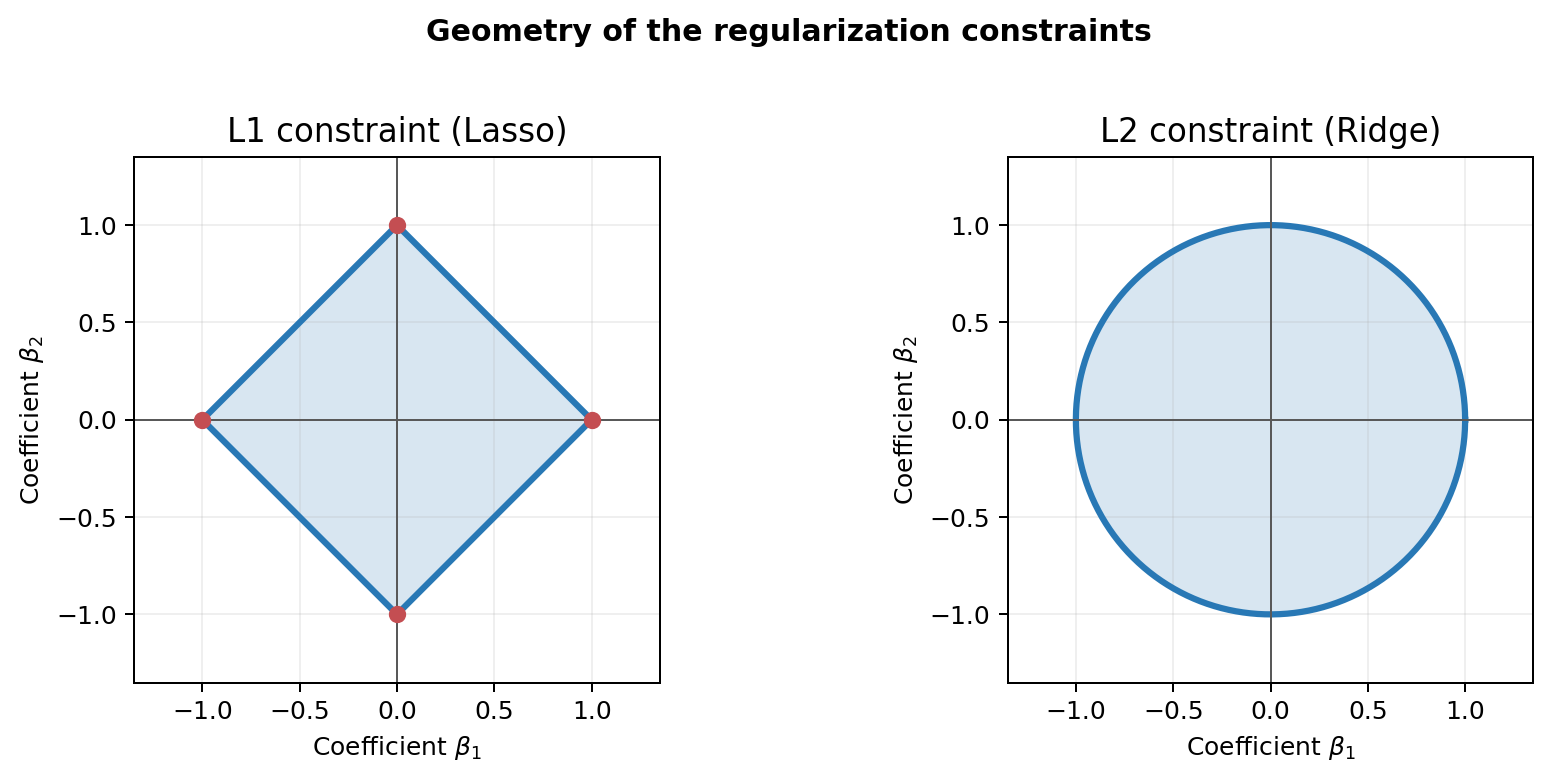
\includegraphics[width=.82\textwidth]{l1_l2_geometry.png}
  \vspace{10mm}
  \begin{tcolorbox}[width=.86\textwidth,colback=PaleBlue,colframe=Blue,arc=2mm,boxrule=.8pt]
    \centering
    \large\bfseries What you will learn\\[3pt]
    \normalsize
    Why Lasso is needed; how the $L_1$ penalty creates sparsity; the geometry and subgradient mathematics; KKT conditions; soft thresholding; coordinate descent; model tuning; correlated predictors; and practical limitations.
  \end{tcolorbox}
  \vfill
  {\large Prepared as a personal revision resource\par}
  \vspace{3mm}
  {\color{Muted}\today\par}
\end{titlepage}

\pagenumbering{roman}
\tableofcontents
\clearpage
\pagenumbering{arabic}

% ==================== 1 INTRO ====================
\chapter{The Big Picture}
\section{What is Lasso Regression?}
Lasso stands for \textbf{Least Absolute Shrinkage and Selection Operator}. It is a regularized linear regression method. Like ordinary least squares (OLS), it tries to predict a response variable from explanatory variables. Unlike OLS, it adds a penalty that discourages large coefficients and can make some coefficients exactly zero.

For $n$ observations and $p$ predictors, write the linear model as
\begin{equation}
  y=X\beta+\varepsilon,
\end{equation}
where $y\in\RR^{n\times1}$ is the response vector, $X\in\RR^{n\times p}$ is the design matrix, $\beta\in\RR^{p\times1}$ is the coefficient vector, and $\varepsilon$ is the error vector. An intercept can be included separately.

\section{Why do we need regularization?}
OLS minimizes the residual sum of squares:
\begin{equation}
  \hat\beta_{\mathrm{OLS}}=\argmin_\beta \norm{y-X\beta}_2^2.
\end{equation}
When predictors are numerous, noisy, or strongly related to one another, an OLS model may have unstable coefficients or overfit the training data. Regularization adds a penalty to the fitting objective to control coefficient size.

\subsection{Ridge versus Lasso}
Ridge uses the squared $L_2$ penalty:
\begin{equation}
  J_{\mathrm{Ridge}}(\beta)=\norm{y-X\beta}_2^2+\lambda\sum_{j=1}^p\beta_j^2.
\end{equation}
Lasso uses the $L_1$ penalty:
\begin{equation}
  \boxed{J_{\mathrm{Lasso}}(\beta)=\norm{y-X\beta}_2^2+\lambda\sum_{j=1}^p\abs{\beta_j}.}
  \label{eq:lasso-objective}
\end{equation}
The parameter $\lambda\geq0$ controls the strength of regularization.

\begin{center}
\begin{tabularx}{.94\textwidth}{>{\bfseries}lXX}
\toprule
Property & Ridge & Lasso\\
\midrule
Penalty & $L_2$: $\sum_j\beta_j^2$ & $L_1$: $\sum_j\abs{\beta_j}$\\
Shrinks coefficients & Yes & Yes\\
Exactly zero coefficients & Not usually & Yes, often\\
Feature selection & Not directly & Built in through sparsity\\
\bottomrule
\end{tabularx}
\end{center}

\begin{keyidea}
Ridge mainly shrinks coefficients toward zero. Lasso shrinks coefficients and can set some of them exactly to zero, producing a sparse model.
\end{keyidea}

\section{What does the tuning parameter $\lambda$ do?}
\begin{itemize}
  \item $\lambda=0$: the penalty disappears and the objective becomes OLS.
  \item A larger $\lambda$: stronger pressure toward smaller coefficients and often more zeros.
  \item An excessively large $\lambda$: useful predictors may also be removed, causing underfitting.
\end{itemize}
The best value is usually selected using validation data or cross-validation, not by looking only at training error.

% ==================== 2 L1 AND GEOMETRY ====================
\chapter{The $L_1$ Penalty and Geometric Intuition}
\section{The $L_1$ norm}
For a coefficient vector $\beta=(\beta_1,\ldots,\beta_p)^T$, its $L_1$ norm is
\begin{equation}
  \norm{\beta}_1=\sum_{j=1}^p\abs{\beta_j}.
\end{equation}
For example, if $\beta=(2,-3,4)^T$, then
\begin{equation}
  \norm{\beta}_1=\abs{2}+\abs{-3}+\abs{4}=9.
\end{equation}
Absolute values ensure that positive and negative coefficients do not cancel each other.

\section{Constraint form and geometry}
The penalized problem can be understood through a constrained form:
\begin{equation}
  \min_\beta \norm{y-X\beta}_2^2
  \quad\text{subject to}\quad \norm{\beta}_1\leq t.
\end{equation}
For two coefficients, the $L_1$ constraint $\abs{\beta_1}+\abs{\beta_2}\leq t$ forms a diamond. The Ridge constraint $\beta_1^2+\beta_2^2\leq t$ forms a circle.
\begin{figure}[htbp]
  \centering
  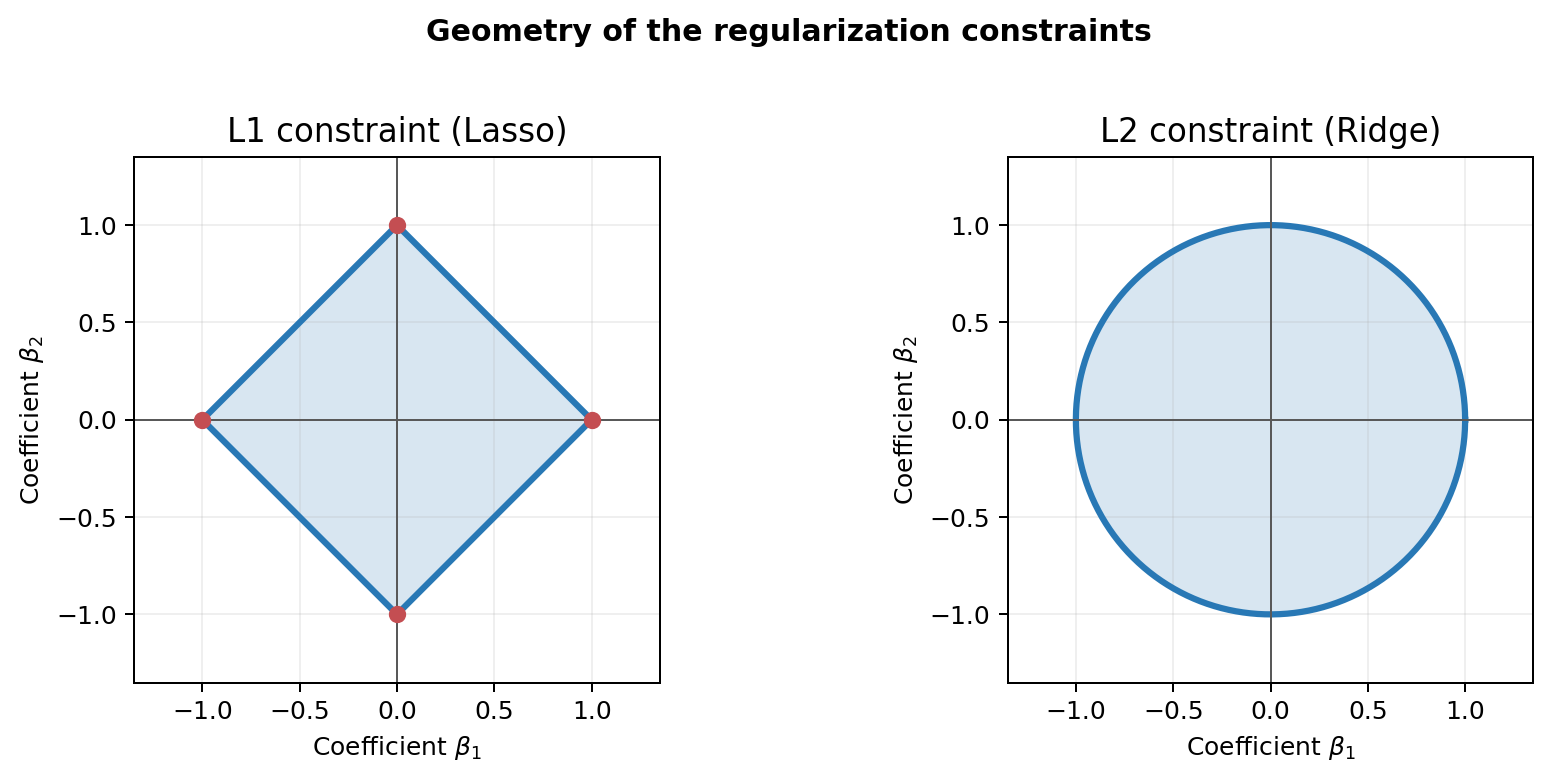
\includegraphics[width=.88\textwidth]{l1_l2_geometry.png}
  \caption{The $L_1$ constraint has sharp corners on the coordinate axes. The $L_2$ constraint is smooth.}
  \label{fig:geometry}
\end{figure}
The contours of the residual sum of squares are ellipses (under a full-rank design). The optimum occurs where the smallest attainable loss contour touches the constraint region. The corners of the $L_1$ diamond lie on the axes, where one coefficient is zero. This makes exact zeros more likely for Lasso.

\begin{intuition}
The geometry gives a visual explanation for sparsity: the sharp corners of the $L_1$ region make a solution with one or more zero coefficients more likely. The smooth $L_2$ boundary does not encourage axis-aligned solutions in the same way.
\end{intuition}

\section{Sparsity}
A vector is sparse when many of its entries are zero. For example,
\begin{equation}
  \hat\beta=(2.1,0,0,2.8,0,-1.1,0,0)^T
\end{equation}
has three nonzero coefficients out of eight. The number of nonzero entries is sometimes denoted by the $L_0$ count:
\begin{equation}
  \norm{\beta}_0=\sum_{j=1}^p I(\beta_j\neq0).
\end{equation}
The $L_0$ count is not a true norm in the strict mathematical sense; it counts nonzero entries. Lasso uses the convex $L_1$ penalty as a computationally convenient way to encourage sparsity.

% ==================== 3 OPTIMIZATION ====================
\chapter{Optimization: From OLS to Lasso}
\section{Why OLS has a closed-form solution}
The OLS objective is
\begin{align}
  J(\beta)&=(y-X\beta)^T(y-X\beta)\\
  &=y^Ty-2\beta^TX^Ty+\beta^TX^TX\beta.
\end{align}
Differentiating,
\begin{equation}
  \nabla_\beta J=-2X^Ty+2X^TX\beta.
\end{equation}
Set the gradient to zero:
\begin{equation}
  X^TX\hat\beta=X^Ty.
\end{equation}
If $X^TX$ is invertible,
\begin{equation}
  \boxed{\hat\beta_{\mathrm{OLS}}=(X^TX)^{-1}X^Ty.}
\end{equation}

\section{Why Ridge also has a closed form}
Ridge adds $\lambda\beta^T\beta$:
\begin{equation}
  J_R(\beta)=(y-X\beta)^T(y-X\beta)+\lambda\beta^T\beta.
\end{equation}
Its gradient is
\begin{equation}
  -2X^Ty+2X^TX\beta+2\lambda\beta.
\end{equation}
Setting it to zero gives
\begin{equation}
  \boxed{\hat\beta_R=(X^TX+\lambda I)^{-1}X^Ty.}
\end{equation}

\section{Why Lasso needs a different optimization method}
Lasso adds $\lambda\sum_j\abs{\beta_j}$. The absolute-value function is not differentiable at zero:
\begin{equation}
  \frac{d}{dx}\abs{x}=\begin{cases}
  1,&x>0,\\-1,&x<0,\\\text{does not exist},&x=0.
  \end{cases}
\end{equation}
Therefore, we cannot simply differentiate the objective in the ordinary way at every point and solve one linear system. Lasso is still a convex optimization problem and can be solved using subgradients, coordinate descent, proximal-gradient methods, and other algorithms.

\section{Subgradients}
A number $g$ is a subgradient of a convex function $f$ at $x$ if
\begin{equation}
  f(z)\geq f(x)+g(z-x)\qquad\text{for every }z.
\end{equation}
For $f(x)=\abs{x}$, the subdifferential is
\begin{equation}
  \boxed{\partial\abs{x}=\begin{cases}
  \{1\},&x>0,\\[-1pt]
  [-1,1],&x=0,\\[-1pt]
  \{-1\},&x<0.
  \end{cases}}
  \label{eq:abs-subgradient}
\end{equation}
At zero, every slope between $-1$ and $1$ is a valid subgradient. This interval is the mathematical feature that allows the optimum to occur exactly at zero.

For the Lasso objective in \cref{eq:lasso-objective}, the subgradient optimality condition is
\begin{equation}
  \boxed{0\in 2X^T(X\hat\beta-y)+\lambda\,\partial\norm{\hat\beta}_1.}
  \label{eq:lasso-subgrad-condition}
\end{equation}
Because the objective is convex, this condition is necessary and sufficient for a global minimum.

% ==================== 4 KKT ====================
\chapter{KKT Optimality Conditions}
\section{Coefficient-wise KKT conditions}
Let $x_j$ denote column $j$ of $X$, and let $r=y-X\hat\beta$ be the residual at the estimated coefficients. The $j$th coordinate of \cref{eq:lasso-subgrad-condition} is
\begin{equation}
  0\in -2x_j^Tr+\lambda\partial\abs{\hat\beta_j}.
\end{equation}
Using the three cases in \cref{eq:abs-subgradient}, we obtain:
\begin{equation}
  \boxed{\begin{array}{ll}
  2x_j^Tr=\lambda,&\hat\beta_j>0,\\[3pt]
  2x_j^Tr=-\lambda,&\hat\beta_j<0,\\[3pt]
  \abs{2x_j^Tr}\leq\lambda,&\hat\beta_j=0.
  \end{array}}
  \label{eq:kkt-piecewise}
\end{equation}
These are the coordinate-wise KKT conditions for the unnormalized RSS convention used throughout this guide.

\begin{keyidea}
For a nonzero coefficient, the residual-feature correlation reaches the positive or negative threshold. For a zero coefficient, its absolute value must be no larger than the threshold. This is the KKT explanation for Lasso's exact zeros.
\end{keyidea}

\section{A small interpretation}
Suppose $\lambda=4$. For a coefficient estimated as zero, the condition is
\begin{equation}
  \abs{2x_j^Tr}\leq4\quad\Longleftrightarrow\quad\abs{x_j^Tr}\leq2.
\end{equation}
If the feature's correlation with the current residual is within this range, the zero coefficient is compatible with optimality. If it is outside the range, that coordinate cannot satisfy the zero-coefficient KKT condition at that point.

\begin{warningbox}
Some books and software use $\frac{1}{2}\RSS+\lambda\norm{\beta}_1$ or $\frac{1}{2n}\RSS+\alpha\norm{\beta}_1$. Their KKT thresholds have different factors. Always derive the condition from the exact objective convention being used.
\end{warningbox}

% ==================== 5 SOFT THRESHOLD ====================
\chapter{Soft Thresholding}
\section{The idea}
Soft thresholding moves values toward zero. Values whose absolute magnitude is no greater than the threshold become exactly zero. Larger values are reduced in magnitude by the threshold.
\begin{equation}
  \boxed{\soft(z,t)=\sign(z)\max(\abs{z}-t,0).}
  \label{eq:soft}
\end{equation}
Equivalently,
\begin{equation}
  \soft(z,t)=\begin{cases}
  z-t,&z>t,\\
  0,&-t\leq z\leq t,\\
  z+t,&z<-t.
  \end{cases}
\end{equation}
\begin{figure}[htbp]
  \centering
  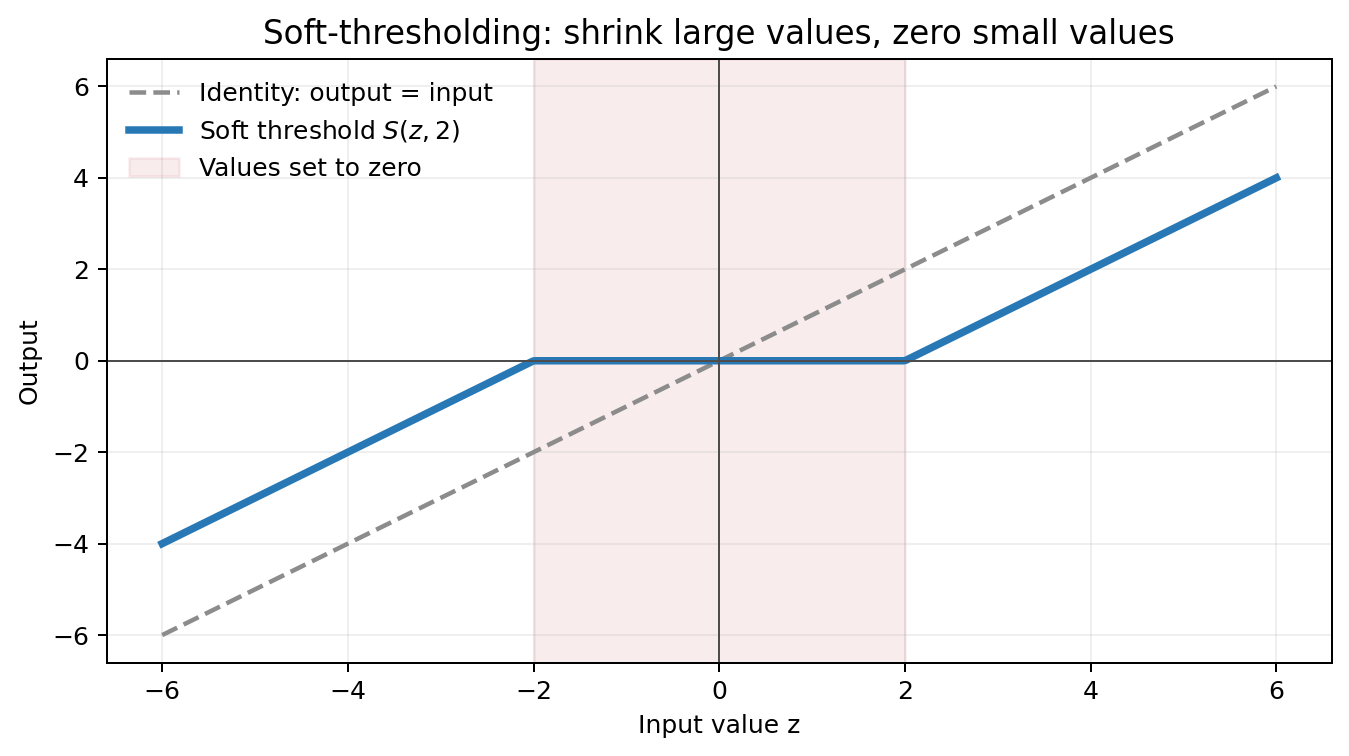
\includegraphics[width=.82\textwidth]{soft_thresholding.png}
  \caption{Soft thresholding with threshold $t=2$. Values in $[-2,2]$ are set to zero.}
  \label{fig:soft}
\end{figure}

\section{Deriving the threshold in an orthonormal case}
Suppose the columns of $X$ are orthonormal, so $X^TX=I$, and define $z=X^Ty$. Ignoring terms independent of $\beta$, the objective separates into
\begin{equation}
  \sum_{j=1}^p\left[(\beta_j-z_j)^2+\lambda\abs{\beta_j}\right].
\end{equation}
For one coordinate, minimize
\begin{equation}
  f(\beta)=(\beta-z)^2+\lambda\abs{\beta}.
\end{equation}
If $\beta>0$, setting the derivative to zero gives $2(\beta-z)+\lambda=0$, hence $\beta=z-\lambda/2$. If $\beta<0$, it gives $2(\beta-z)-\lambda=0$, hence $\beta=z+\lambda/2$. At $\beta=0$, the subgradient condition holds when $\abs{z}\leq\lambda/2$. Combining the cases,
\begin{equation}
  \boxed{\hat\beta_j=\soft(z_j,\lambda/2).}
\end{equation}

\begin{worked}
Let $t=2$. Then $\soft(5,2)=3$, $\soft(-5,2)=-3$, and $\soft(1.5,2)=0$. Large values shrink; small values disappear.
\end{worked}

\begin{warningbox}
The threshold is $\lambda/2$ here because the objective uses unnormalized RSS, $\RSS+\lambda\norm{\beta}_1$. If the loss is $\frac12\RSS+\lambda\norm{\beta}_1$, the threshold is $\lambda$.
\end{warningbox}

% ==================== 6 COORDINATE DESCENT ====================
\chapter{Coordinate Descent}
\section{What is coordinate descent?}
Coordinate descent is an iterative optimization algorithm. Instead of updating all coefficients simultaneously, it updates one coefficient at a time while holding the other coefficients fixed. It cycles through the features until the solution changes very little.

\begin{figure}[htbp]
  \centering
  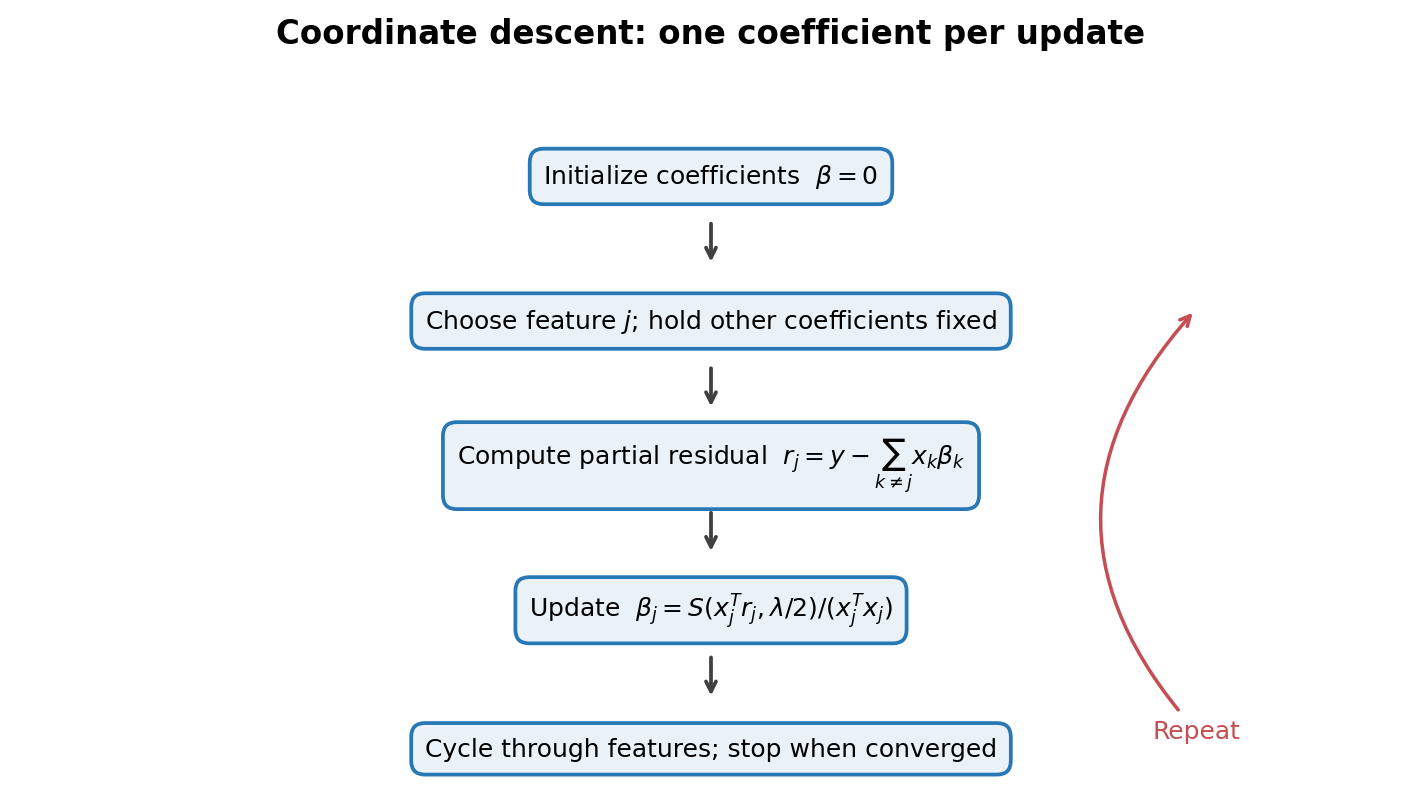
\includegraphics[width=.73\textwidth]{coordinate_descent_flow.png}
  \caption{The basic coordinate-descent workflow for Lasso.}
  \label{fig:cd-flow}
\end{figure}

\section{Deriving the coordinate update}
Start with
\begin{equation}
  J(\beta)=\norm{y-X\beta}_2^2+\lambda\sum_{k=1}^p\abs{\beta_k}.
\end{equation}
To update coefficient $\beta_j$, hold all other coefficients fixed and define the partial residual
\begin{equation}
  \boxed{r_j=y-\sum_{k\neq j}x_k\beta_k.}
\end{equation}
Then $y-X\beta=r_j-x_j\beta_j$. The part of the objective that depends on $\beta_j$ is
\begin{align}
  f(\beta_j)&=\norm{r_j-x_j\beta_j}_2^2+\lambda\abs{\beta_j}+\text{constant}\\
  &=\beta_j^2x_j^Tx_j-2\beta_jx_j^Tr_j+\lambda\abs{\beta_j}+\text{constant}.
\end{align}
Define
\begin{equation}
  a_j=x_j^Tx_j,\qquad z_j=x_j^Tr_j.
\end{equation}
Then
\begin{equation}
  f(\beta_j)=a_j\beta_j^2-2z_j\beta_j+\lambda\abs{\beta_j}+\text{constant}.
\end{equation}
Completing the square and applying soft thresholding gives
\begin{equation}
  \boxed{\beta_j^{\mathrm{new}}=\frac{\soft(z_j,\lambda/2)}{a_j}
  =\frac{\soft(x_j^Tr_j,\lambda/2)}{x_j^Tx_j}.}
  \label{eq:coordinate-update}
\end{equation}

\section{Numerical coordinate update}
Suppose $x_j^Tr_j=7$, $x_j^Tx_j=4$, and $\lambda=2$. Then the threshold is $\lambda/2=1$:
\begin{align}
  \soft(7,1)&=6,\\
  \beta_j^{\mathrm{new}}&=\frac{6}{4}=1.5.
\end{align}
If instead $x_j^Tr_j=0.5$, then $\soft(0.5,1)=0$, so the updated coefficient is exactly zero.

\section{Algorithm in pseudocode}
\begin{tcolorbox}[colback=black!3,colframe=Muted!70,arc=2mm,boxrule=.5pt]
\ttfamily\small
Initialize beta = (0, ..., 0)\par
Repeat until convergence:\par
\quad For j = 1, ..., p:\par
\qquad r = y - X beta + x\_j beta\_j\par
\qquad z = x\_j\^T r\par
\qquad a = x\_j\^T x\_j\par
\qquad beta\_j = SoftThreshold(z, lambda/2) / a\par
\end{tcolorbox}
The residual expression $r=y-X\beta+x_j\beta_j$ removes the current contribution of feature $j$ from the fitted values, leaving the partial residual for that coordinate. The algorithm then updates $\beta_j$ and moves to the next feature.

\section{When does the algorithm stop?}
A practical stopping rule is
\begin{equation}
  \max_j\abs{\beta_j^{(t+1)}-\beta_j^{(t)}}<\epsilon,
\end{equation}
where $\epsilon$ is a small tolerance. Implementations may also monitor objective changes or KKT violations. Since the Lasso objective is convex, coordinate descent converges to a global minimizer under standard conditions; if the minimizer is not unique, different coefficient vectors can attain the same minimum.

\section{How coordinate descent and KKT connect}
Coordinate descent is a method for finding coefficients. KKT conditions characterize whether the coefficients are optimal. At convergence, each coordinate should satisfy the corresponding condition in \cref{eq:kkt-piecewise}. Practical solvers check these conditions numerically to assess convergence.

% ==================== 7 PRACTICAL MODELING ====================
\chapter{Practical Modeling: Scaling and Choosing $\lambda$}
\section{Why standardize predictors?}
Lasso penalizes coefficient magnitudes. Coefficient magnitudes depend on the units in which predictors are measured. For example, income measured in dollars has a different numerical scale from age measured in years. Without scaling, the penalty can affect features unevenly simply because of their units.

A common standardization is
\begin{equation}
  z_{ij}=\frac{x_{ij}-\mu_j}{s_j},
\end{equation}
where $\mu_j$ and $s_j$ are the training-set mean and standard deviation of feature $j$. After this transformation, each predictor has approximately zero mean and unit standard deviation.

\begin{keyidea}
Fit the scaler on the training data only. Apply the same training means and standard deviations to validation and test data. This avoids data leakage.
\end{keyidea}

The intercept is usually not penalized. A common approach is to center the predictors and response, fit the penalized slopes, and estimate the intercept separately.

\section{Choosing lambda with cross-validation}
A larger $\lambda$ often produces a simpler model, but too much regularization can underfit. A common approach is $K$-fold cross-validation. Split the training data into $K$ folds; train on $K-1$ folds and validate on the remaining fold; repeat so each fold is used for validation; average the validation errors for each candidate $\lambda$.
\begin{figure}[htbp]
  \centering
  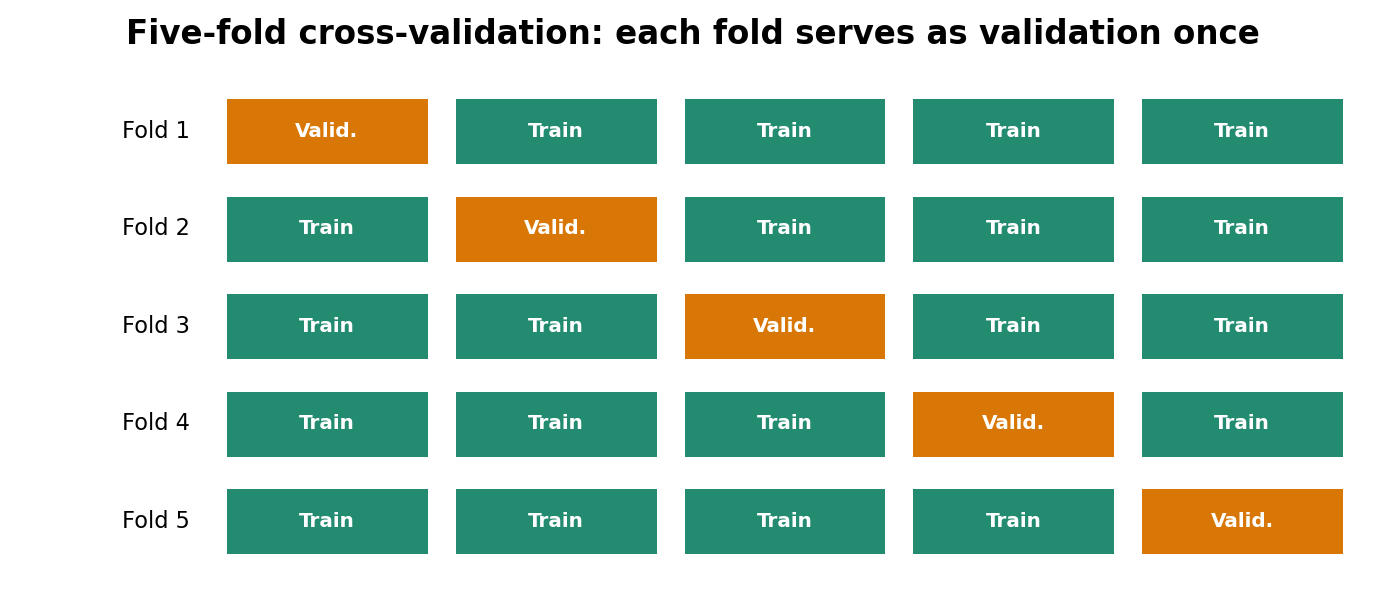
\includegraphics[width=.82\textwidth]{five_fold_cv.png}
  \caption{Five-fold cross-validation. Each fold is used as the validation fold once.}
  \label{fig:cv}
\end{figure}
Choose the $\lambda$ with the best average validation performance, or use a simplicity-oriented rule such as the one-standard-error rule. The final test set should be reserved for a final evaluation after model selection.

\section{Regularization paths}
A regularization path shows how each estimated coefficient changes as $\lambda$ changes. The horizontal axis is often $\lambda$ on a logarithmic scale, and each curve represents one coefficient.
\begin{figure}[htbp]
  \centering
  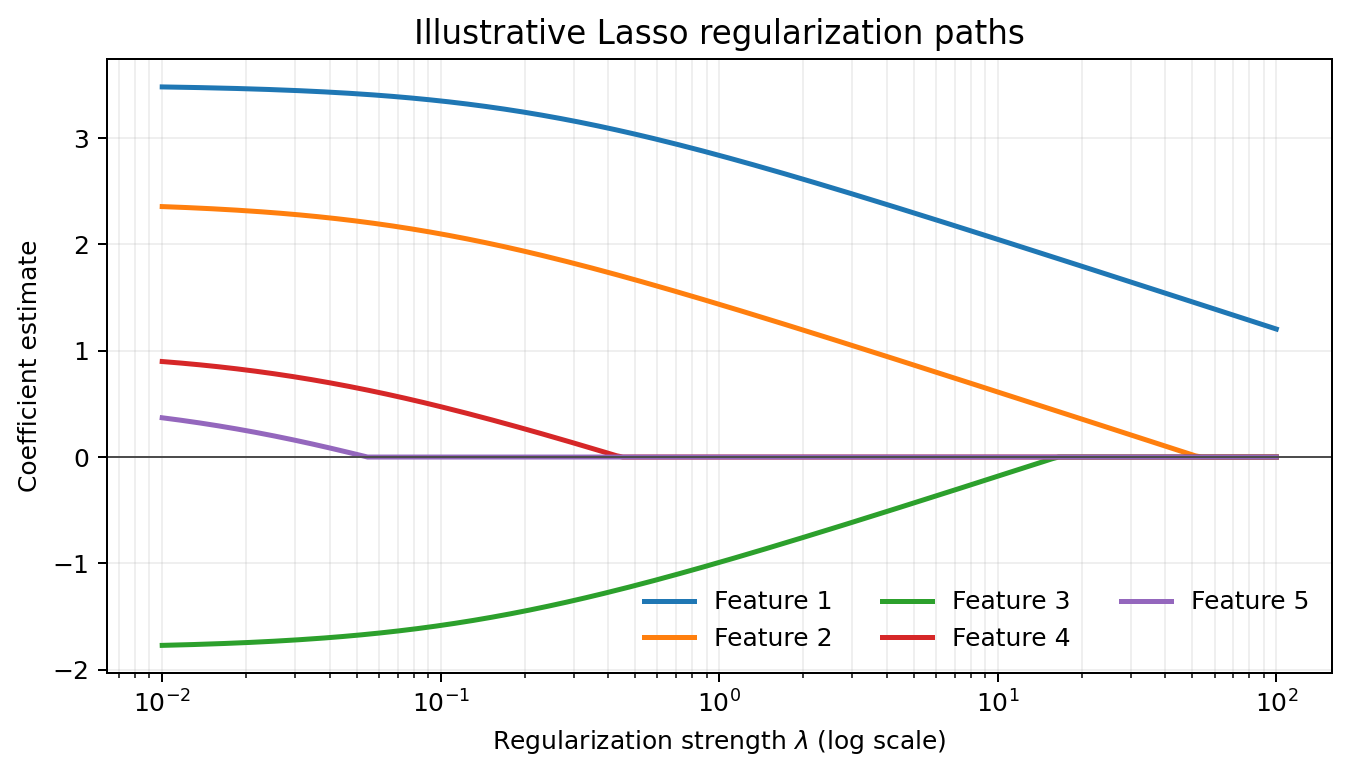
\includegraphics[width=.82\textwidth]{regularization_path.png}
  \caption{Illustrative coefficient paths as regularization becomes stronger. This is a conceptual illustration, not empirical data.}
  \label{fig:path}
\end{figure}
As regularization becomes stronger, coefficients generally move toward zero. A path can reveal which variables remain active over a range of penalty strengths.

\section{The all-zero threshold}
Assume predictors and response are centered and use the unnormalized objective in \cref{eq:lasso-objective}. At $\beta=0$, the KKT condition for every coefficient is
\begin{equation}
  \abs{2x_j^Ty}\leq\lambda.
\end{equation}
Thus a threshold at which the all-zero coefficient vector is optimal is
\begin{equation}
  \boxed{\lambda_{\max}=2\max_j\abs{x_j^Ty}.}
\end{equation}
This formula changes if the loss is scaled differently. If an intercept is present, centering is one way to handle it separately.

% ==================== 8 ADVANCED ====================
\chapter{Advanced Concepts: Strengths and Limitations}
\section{Sparsity and feature selection}
Lasso can set some estimated coefficients exactly to zero. This provides a form of feature selection and can make a model easier to interpret. However, a zero coefficient means that the fitted model did not retain that feature under the chosen data, penalty, and other predictors. It does not prove that the feature is scientifically irrelevant or has no causal effect.

\section{Correlated predictors}
Suppose two predictors contain almost the same information. Lasso may retain one and set the other to zero. With perfectly identical columns, multiple coefficient allocations can produce the same predictions and the same $L_1$ penalty. With highly correlated but not identical columns, the selected feature can be sensitive to small changes in the data.

Ridge often distributes coefficient weight across correlated predictors because the squared $L_2$ penalty can be smaller when weight is spread across them. Elastic Net combines both penalties:
\begin{equation}
  J_{\mathrm{EN}}(\beta)=\RSS(\beta)+\lambda_1\norm{\beta}_1+\lambda_2\norm{\beta}_2^2.
\end{equation}
The $L_1$ term encourages sparsity; the $L_2$ term encourages more stable, shared shrinkage among correlated predictors.

\section{Limitations of Lasso}
\begin{enumerate}
  \item \textbf{Unstable selection among correlated predictors.} Small changes in the sample can change which member of a correlated group is selected.
  \item \textbf{Regularization bias.} Shrinking coefficients toward zero introduces bias, even for predictors that truly matter.
  \item \textbf{Over-regularization.} A very large $\lambda$ can remove useful predictors and underfit.
  \item \textbf{Scaling sensitivity.} Predictors should generally be standardized so that units do not dominate the penalty.
  \item \textbf{No causal guarantee.} Predictive feature selection does not establish causation.
  \item \textbf{Dense true models.} If many predictors genuinely have small nonzero effects, Lasso may remove some of them; Ridge may be more appropriate.
  \item \textbf{High-dimensional selection limit.} Under common general-position conditions, a Lasso solution with $n$ observations selects no more than $n$ predictors. This can matter when the number of predictors greatly exceeds the sample size.
\end{enumerate}

% ==================== 9 SUMMARY ====================
\chapter{Revision Sheet and Self-Test}
\section{The essential formulas}
\begin{align*}
  \text{Lasso objective:}\quad&\RSS+\lambda\norm{\beta}_1\\
  \text{$L_1$ norm:}\quad&\norm{\beta}_1=\sum_j\abs{\beta_j}\\
  \text{Absolute-value subgradient:}\quad&\partial\abs{x}=\begin{cases}\{1\},&x>0\\[-2pt][-1,1],&x=0\\[-2pt]\{-1\},&x<0\end{cases}\\
  \text{Lasso optimality:}\quad&0\in2X^T(X\hat\beta-y)+\lambda\partial\norm{\hat\beta}_1\\
  \text{Soft threshold:}\quad&\soft(z,t)=\sign(z)\max(\abs{z}-t,0)\\
  \text{Coordinate update:}\quad&\beta_j^{\mathrm{new}}=\frac{\soft(x_j^Tr_j,\lambda/2)}{x_j^Tx_j}.
\end{align*}

\section{Conceptual summary}
\begin{itemize}
  \item Lasso is linear regression with an $L_1$ penalty.
  \item The $L_1$ penalty encourages sparse coefficient vectors.
  \item The absolute value is not differentiable at zero, so subgradients are used.
  \item KKT conditions characterize the optimal coefficient pattern.
  \item Soft thresholding shrinks large values and sets sufficiently small values to zero.
  \item Coordinate descent updates one coefficient at a time using partial residuals.
  \item Standardization and cross-validation are important for practical modeling.
  \item Correlated predictors and regularization bias are important limitations.
\end{itemize}

\section{Self-test questions}
\begin{enumerate}
  \item What is the difference between Ridge and Lasso penalties?
  \item Why can Lasso produce exact zeros?
  \item Why is the ordinary derivative of $\abs{x}$ unavailable at $x=0$?
  \item State the three coefficient-wise KKT cases for Lasso.
  \item What does soft thresholding do when $\abs{z}\leq t$?
  \item Why does coordinate descent use a partial residual?
  \item Derive the coordinate update formula from the one-coordinate objective.
  \item Why should predictors generally be standardized before fitting Lasso?
  \item How does cross-validation help select $\lambda$?
  \item Why can highly correlated predictors make Lasso feature selection unstable?
\end{enumerate}

\section{Short answers}
\begin{enumerate}
  \item Ridge uses an $L_2$ squared penalty; Lasso uses an $L_1$ absolute-value penalty.
  \item The $L_1$ penalty has a subgradient interval at zero, and its geometry has corners on the coordinate axes.
  \item The left and right derivatives at zero differ ($-1$ and $+1$).
  \item Positive: $2x_j^Tr=\lambda$; negative: $2x_j^Tr=-\lambda$; zero: $\abs{2x_j^Tr}\leq\lambda$.
  \item It returns zero.
  \item The partial residual removes the current contribution of feature $j$, isolating the one-dimensional update.
  \item Expand the one-coordinate objective, complete the square, and apply soft thresholding.
  \item The penalty acts on coefficient magnitudes, which depend on predictor units.
  \item It estimates out-of-sample performance for candidate penalty values.
  \item Similar predictors can substitute for one another, so one may be selected while another is discarded.
\end{enumerate}

\begin{keyidea}[title=One final mental model]
Lasso balances fit and simplicity. The residual term asks the model to explain the data; the $L_1$ term asks it to keep coefficient magnitudes under control. Subgradients and KKT conditions describe the optimum, soft thresholding explains zero coefficients, and coordinate descent is a practical way to find them.
\end{keyidea}

\end{document}
